\documentclass[a4paper,english,11pt]{article}
\usepackage[T1]{fontenc}
\usepackage[latin1]{inputenc}
\usepackage{babel}
\usepackage{times}
\usepackage{graphicx}
\usepackage{url}
\usepackage[right=2.5cm,left=2.5cm,top=2.5cm,bottom=2.5cm,nohead]{geometry}

\newcommand{\fig}[3][htbp]{
  \begin{figure}[#1] {\centering\scalebox{0.75}{\includegraphics{fig/#2}}\par}
    \caption{#3\label{fig:#2}}
  \end{figure}
}

\title{An Application-Oriented Communication System for Clusters of Workstations}

\author{Thiago Robert C. Santos and Antonio Augusto Frohlich}

\date{\small Laboratory for Software/Hardware Integration (LISHA)\\
  Federal University of Santa Catarina (UFSC)\\
  88049-900 Florianopolis - SC - Brazil\\
  PO Box 476\\
  Phone: +55 48 331-7552~~~~Fax: +55 48 331-9770\\
  \{robert | guto\}@lisha.ufsc.br\\
  http://www.lisha.ufsc.br/$\sim$\{robert | guto\}
}

\begin{document} 

\maketitle

\begin{abstract}
  
The present paper proposes an application-oriented communication sub-system to be used in \textsc{Snow}, a high-performance, application-oriented parallel-programming environment for dedicated clusters. The proposed communication sub-system is composed of a baseline architecture and a family of lightweight network interface protocols. Each one of these protocols is built on top of the baseline architecture and can be tailored in order to satisfy the needs of specific classes of parallel applications. The family of lightweight protocols, along with the baseline architecture that supports it, consists of a customizable component in \textsc{Epos}, an application-oriented, component-based operating system that is the core of \textsc{Snow}. The idea behind providing a set of low-level protocol implementations instead of a single monolithic protocol is that parallel applications running on dedicated clusters can improve their communication performance by using the most appropriate protocol for their needs.

\paragraph{Keywords:} lightweight communication protocols, application-oriented operating systems, user-level communication.

\end{abstract}

%%%%%%%%%%%%%%%%%%%%%%%%%%%%%%%%%%%%%%%%%%%%%%%%%%%%%%%%%%%%%%%%%%%%%%%%%%%%%%%
\section{Introduction\label{sec:intro}}

\emph{Clusters of commodity workstations} are now commonplace in \emph{high-performance computing}. In fact, commercial off-the-shelf processors and high-speed networks evolved so much in recent years that most of the hardware features once used to characterize \emph{massively parallel processors}~(MPP) are now available in clusters as well. Nonetheless, the majority of the clusters in use today rely on commodity run-time support systems (run-time libraries, operating systems, compilers, etc.) that have usually been designed in disregard of both parallel applications and hardware. In such systems, delivering a parallel API like MPI is usually achieved through a series of patches or middleware layers that invariably add on overhead for applications. Therefore, it seems logical to suppose that a run-time support system specially designed to support parallel applications on clusters of workstations could considerably improve on performance and also on other software quality metrics (e.g. usability, correctness, adaptability).

Our supposition that ordinary run-time support systems are inadequate to support high-performance computing is sustained by a number of research projects in the field focusing on the implementation of \emph{message passing}~\cite{Gropp:1996,Burns:1994} and \emph{shared memory}~\cite{Bershad:1991,Cordsen:1996, Hellwagner:1995} middlewares and on \emph{user-level communication}~\cite{Prylli:1998,Lumetta:1997, Tezuka:1997}. If ordinary operating systems could match with parallel application's needs, delivering adequate run-time support for the most traditional programming paradigms with minimum overhead, many of theses researches would be hard to justify outside the realm of operating systems. Indeed, the way ordinary operating systems handle I/O is largely based on multitasking concepts such as domain protection and resource sharing. This impacts the way recurring operations like system calls, CPU scheduling, and application's data management are implemented, making little room for novel technological features~\cite{ccwp}. Not surprisingly, system designers often have to push the operating system out of the way in order to implement efficient schedulers and communication systems for clusters.

Besides, commodity operating systems usually target reconfigurability at standard conformance and device support, failing to comply with applications' requirements. Clusters have been quenching the industry's thirst for low-end supercomputers for years as HPC service providers deploy cost-effective solutions based on cluster systems. There are all kinds of applications running on clusters today, ranging from communication-intensive distributed databases to CPU-hungry scientific applications. Having the chance to customize a cluster's run-time support system to satisfy particular applications' needs could improve the system's overall performance. Indeed, systems such as \textsc{Peace}~\cite{Preikschat:1994} and \textsc{Choices}~\cite{Campbell:1992} have already confirmed this hypothesis in the 90s.

In this paper, we discuss the use of dedicated run-time support system, or, more specifically, of \emph{dedicated communication systems}, as effective alternatives to support communication-intensive parallel applications in clusters of workstations. The research that subsided this discussion was carried out in the scope of the \textsc{Snow} project~\cite{Froehlich:gbwit:2000}, which aims at developing a high-performance, application-oriented parallel-programming environment for dedicated clusters. Actually, \textsc{Snow}'s run-time system comes from another project, namely \textsc{Epos}, which takes on a repository of software components, an adaptive component framework, and a set of tools to build application-oriented operating systems on demand~\cite{Froehlich:sbac:1999}.

The remainder of this paper is structured as follows. Section~\ref{sec:Epos} gives an overview of \textsc{Epos}. Section~\ref{sec:commsys} presents a redesign of \textsc{Epos} communication system aimed at enhancing support for \emph{network interface protocols} and describes the baseline architecture that supports these protocols. Section~\ref{sec:related} elaborates on related works. Conclusions are presented in Section~\ref{sec:end}, along with the directions for future work.

%%%%%%%%%%%%%%%%%%%%%%%%%%%%%%%%%%%%%%%%%%%%%%%%%%%%%%%%%%%%%%%%%%%%%%%%%%%%%%%
\section{An Overview of \textsc{Epos}\label{sec:Epos}}

\textsc{Epos}, the \emph{Embedded Parallel Operating System}, is a highly customizable operating system developed using state-of-the-art software engineering techniques. \textsc{Epos} consists of a collection of reusable and adaptable software components and a set of tools that support parallel application developers in ``plugging'' these components into an adaptive framework to produce a variety of run-time systems, including complete operating systems. Being fruit of \emph{Application-Oriented System Design}~\cite{Froehlich:2001}, method that covers the development of application-oriented operating systems from domain analysis to implementation, \textsc{Epos} can be customized to match the requirements of particular parallel applications. \textsc{Epos} components, or scenario-independent system abstractions as they are called, are grouped in families and kept independent of execution scenario by deploying aspect separation and other factorization techniques during the domain engineering process (figure~\ref{fig:aosd} illustrates this process). \textsc{Epos} components can be adapted to be reused in a variety of execution scenarios. Usability is largely improved by hiding the details of a family of abstraction behind an hypothetical interface, called the family's \emph{inflated interface}, and delegating the selection of proper family members to automatic configuration tools.

\begin{figure} [h]
\centering
\fbox{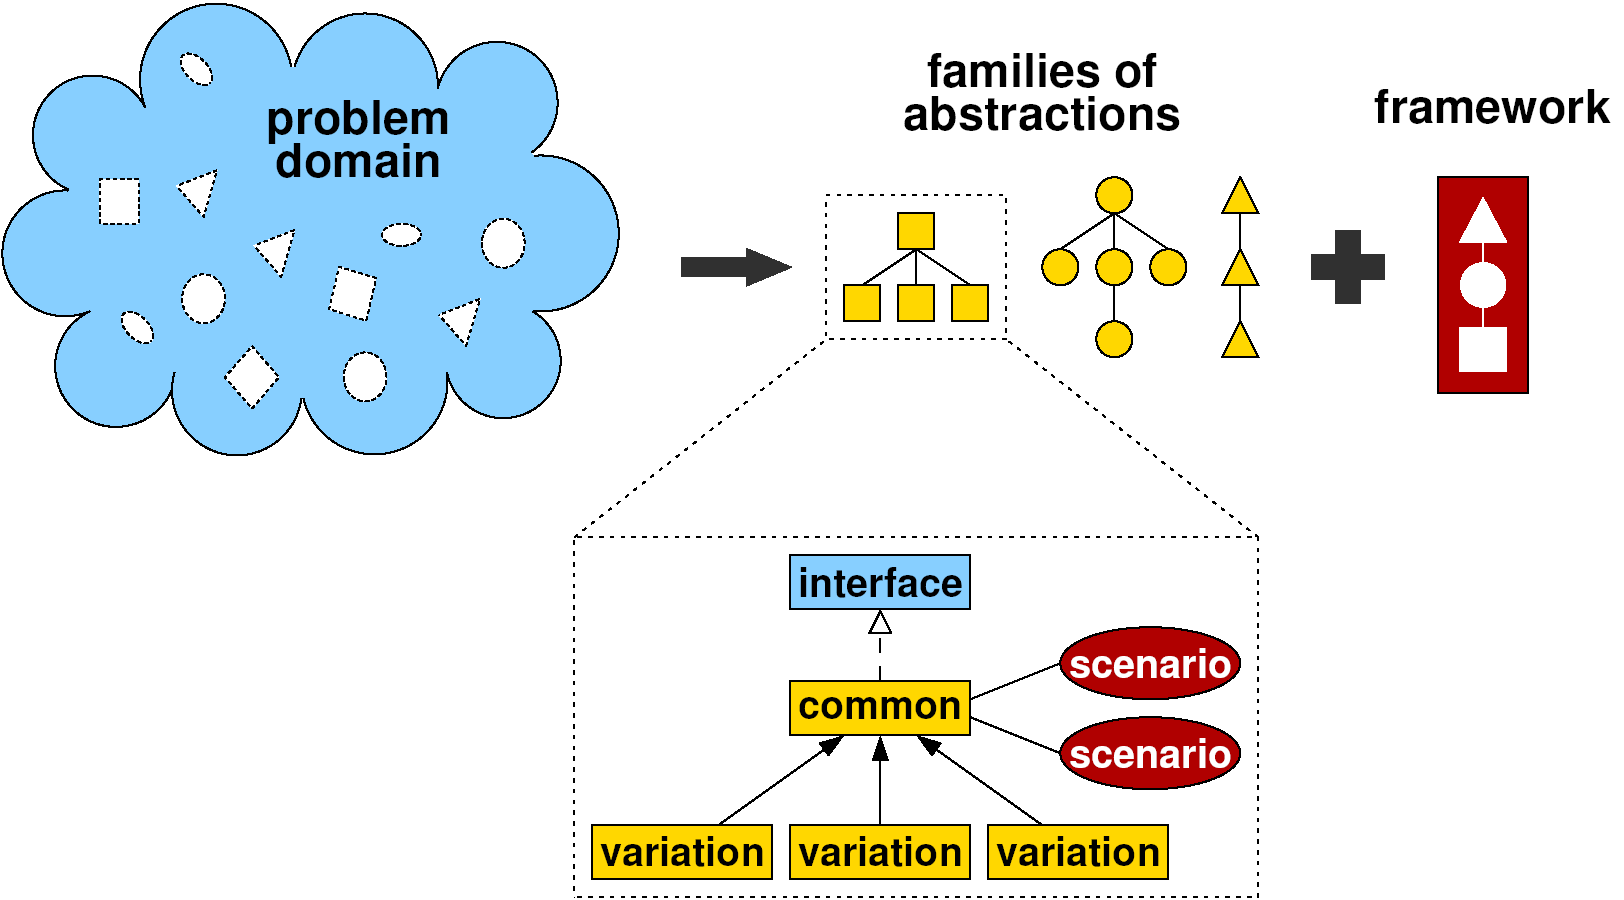
\includegraphics[scale=0.75]{fig/aosd}}
\caption{An overview of \emph{Application-Oriented System Design}.}
\label{fig:aosd}
\end{figure}

An application written based on inflated interfaces can be submitted to a tool that scans it searching for references to the interfaces, thus rendering the features of each family that are necessary to support the application at run-time. This tool, the \texttt{analyzer}, outputs a specification of requirements in the form of partial component interface declarations, including methods, types and constants that were used by the application. 

The primary specification produced by the analyzer is subsequently fed into a second tool, the \texttt{configurator}, that consults a build-up database to further refine the specification. This database holds information about each component in the repository, as well as dependencies and composition rules that are used by the configurator to build a dependency tree. Additionally, each component in the repository is tagged with a ``cost'' estimation, so that the configurator will chose the ``cheapest'' option whenever two or more components satisfy a dependency. The output of the configurator consists of a set of keys that define the binding of inflated interfaces to abstractions and activate the scenario aspects and configurable features eventually identified as necessary to satisfy the constraints dictated by the target application or by the configured execution scenario.

\begin{figure} [h]
\centering
\fbox{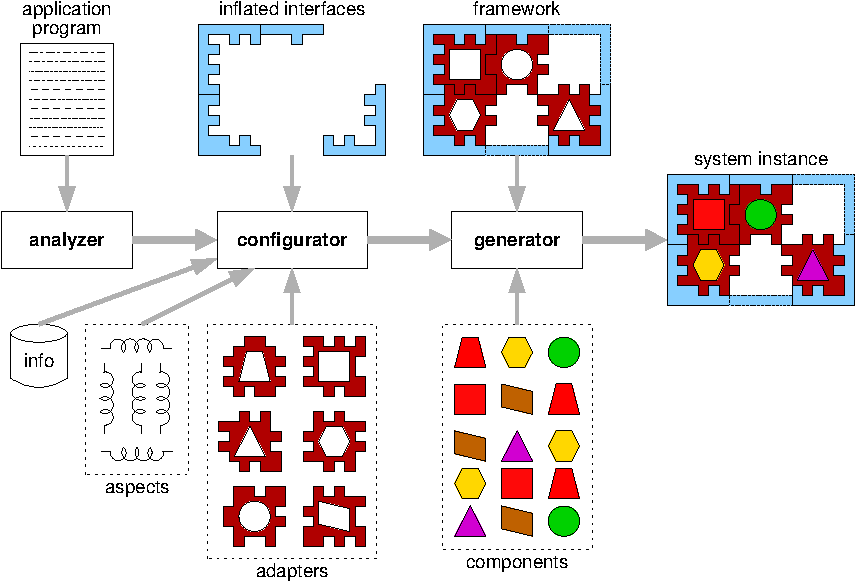
\includegraphics[scale=0.75]{fig/tools}}
\caption{An overview of \textsc{Epos} generation tools.}
\label{fig:tools}
\end{figure}

The last step in run-time systems generation process is accomplished by the \texttt{generator}. This tool translates the keys produced by the configurator into parameters for a statically meta programed component framework and triggers the compilation of a tailored system instance. Figure~\ref{fig:tools} brings an overview of the whole procedure.

%%%%%%%%%%%%%%%%%%%%%%%%%%%%%%%%%%%%%%%%%%%%%%%%%%%%%%%%%%%%%%%%%%%%%%%%%%%%%%%
\section{\textsc{Epos} Communication System\label{sec:commsys}}

\textsc{Epos} communication system is designed around three major families of abstractions: communicator, channel, and network. The \texttt{communicator} family encompasses communication end-points such as link, port, and mailbox, thus acting as the main interface between the communication system and application programs\footnote{The component nature of \textsc{Epos} enables individual elements of the communication system to be reused in isolation, even directly by applications. Therefore, the communicator is not the only visible interface in the communication system.}. The second family, \texttt{channel}, features communication protocols, so that application data fed into the communication system via a communicator gets delivered at the destination communicator accordingly. A channel implements a communication protocol that, according to the ISO/OSI-RM reference would be classified at level four (transport). The third family in \textsc{Epos} communication system, \texttt{network}, is responsible for abstracting distinct network technologies through a common interface\footnote{Each member in the network family is allowed to extend this interface to account for advanced features.}, thus keeping the communication system itself architecture-independent and allowing for flexible combinations of protocols and network architectures.

\fig{epos_comm}{An overview of \textsc{Epos} communication system.}

Previous partial implementations of \textsc{Epos} communication system for the \emph{Myrinet} high-speed network architecture confirmed the lightness of its core, delivering unprecedented bandwidth and latency to parallel applications running on \textsc{Snow}~\cite{Froehlich:ccgrid:2001}. Nonetheless, \textsc{Epos} communication system original designs makes it hard to split the implementation of \emph{network interface protocols}~\cite{bhoedjang98niprotocols} between the processors in the host machine and in the network adapter. Besides, it is very difficult to specify a single network interface protocol that is optimal for all parallel application, since different applications impose different traffic patterns on the underlying network. Instead of developing a single, highly complex, all encompassing protocol, it appears more feasible to construct an architecture that permits fine-grain selection and dynamic configuration of precisely specified \emph{low-level lightweight protocol} mechanisms. In an application-oriented environment, this set of low-level protocols can be used to customize communication according to applications' needs.

\textsc{Epos} design allows for the several network interface protocols that arise from the design decisions related to network features to be grouped into a software component with a defined interface, a \emph{family}, that can be easily accessed by the communication system of the OS. \textsc{Epos}' framework implements mechanisms for fine-grain selection of modules according to applications' needs. These same mechanisms can be used to select the low-level lightweight protocols that better satisfy the applications' communications requirements. Besides, an important step towards an efficient, application-oriented communication system for clusters is to better understand the relation between the design decisions in low-level communication software and the performance of high-level applications. Grouping the different low-level implementations of communication protocols in a component coupled with the communication system has the additional advantage of allowing an application to experiment with different communications schemes, collecting metrics in order to identify the best scheme for its needs. In addition to that, to structure communication in such a modular fashion enhances maintainability and extensibility.

%%%%%%%%%%%%%%%%%%%%%%%%%%%%%%%%%%%%%%%%%%%%%%%%%%%%%%%%%%%%%%%%%%%%%%%%%%%%%%%
\subsection{Myrinet baseline architecture}

The baseline communication architecture that supports the low-level lightweight protocols for the Myrinet networking technology must be simple and flexible enough not to hinder the design and implementation of specific protocols. The highest bandwidth and lowest latency possible are desired since complex protocol implementations will definitely affect both of them. User-level communication was the best answer from academia to the lack of efficient communication protocols for modern, high-performance networks. The baseline architecture described in this section follows the general concepts behind successful user-level communication systems for Myrinet. Figure \ref{fig:best_design} exhibits this architecture, highlighting the data flow during communication as well as host and NIC memory layout.

\begin{figure} [h]
\centering
\fbox{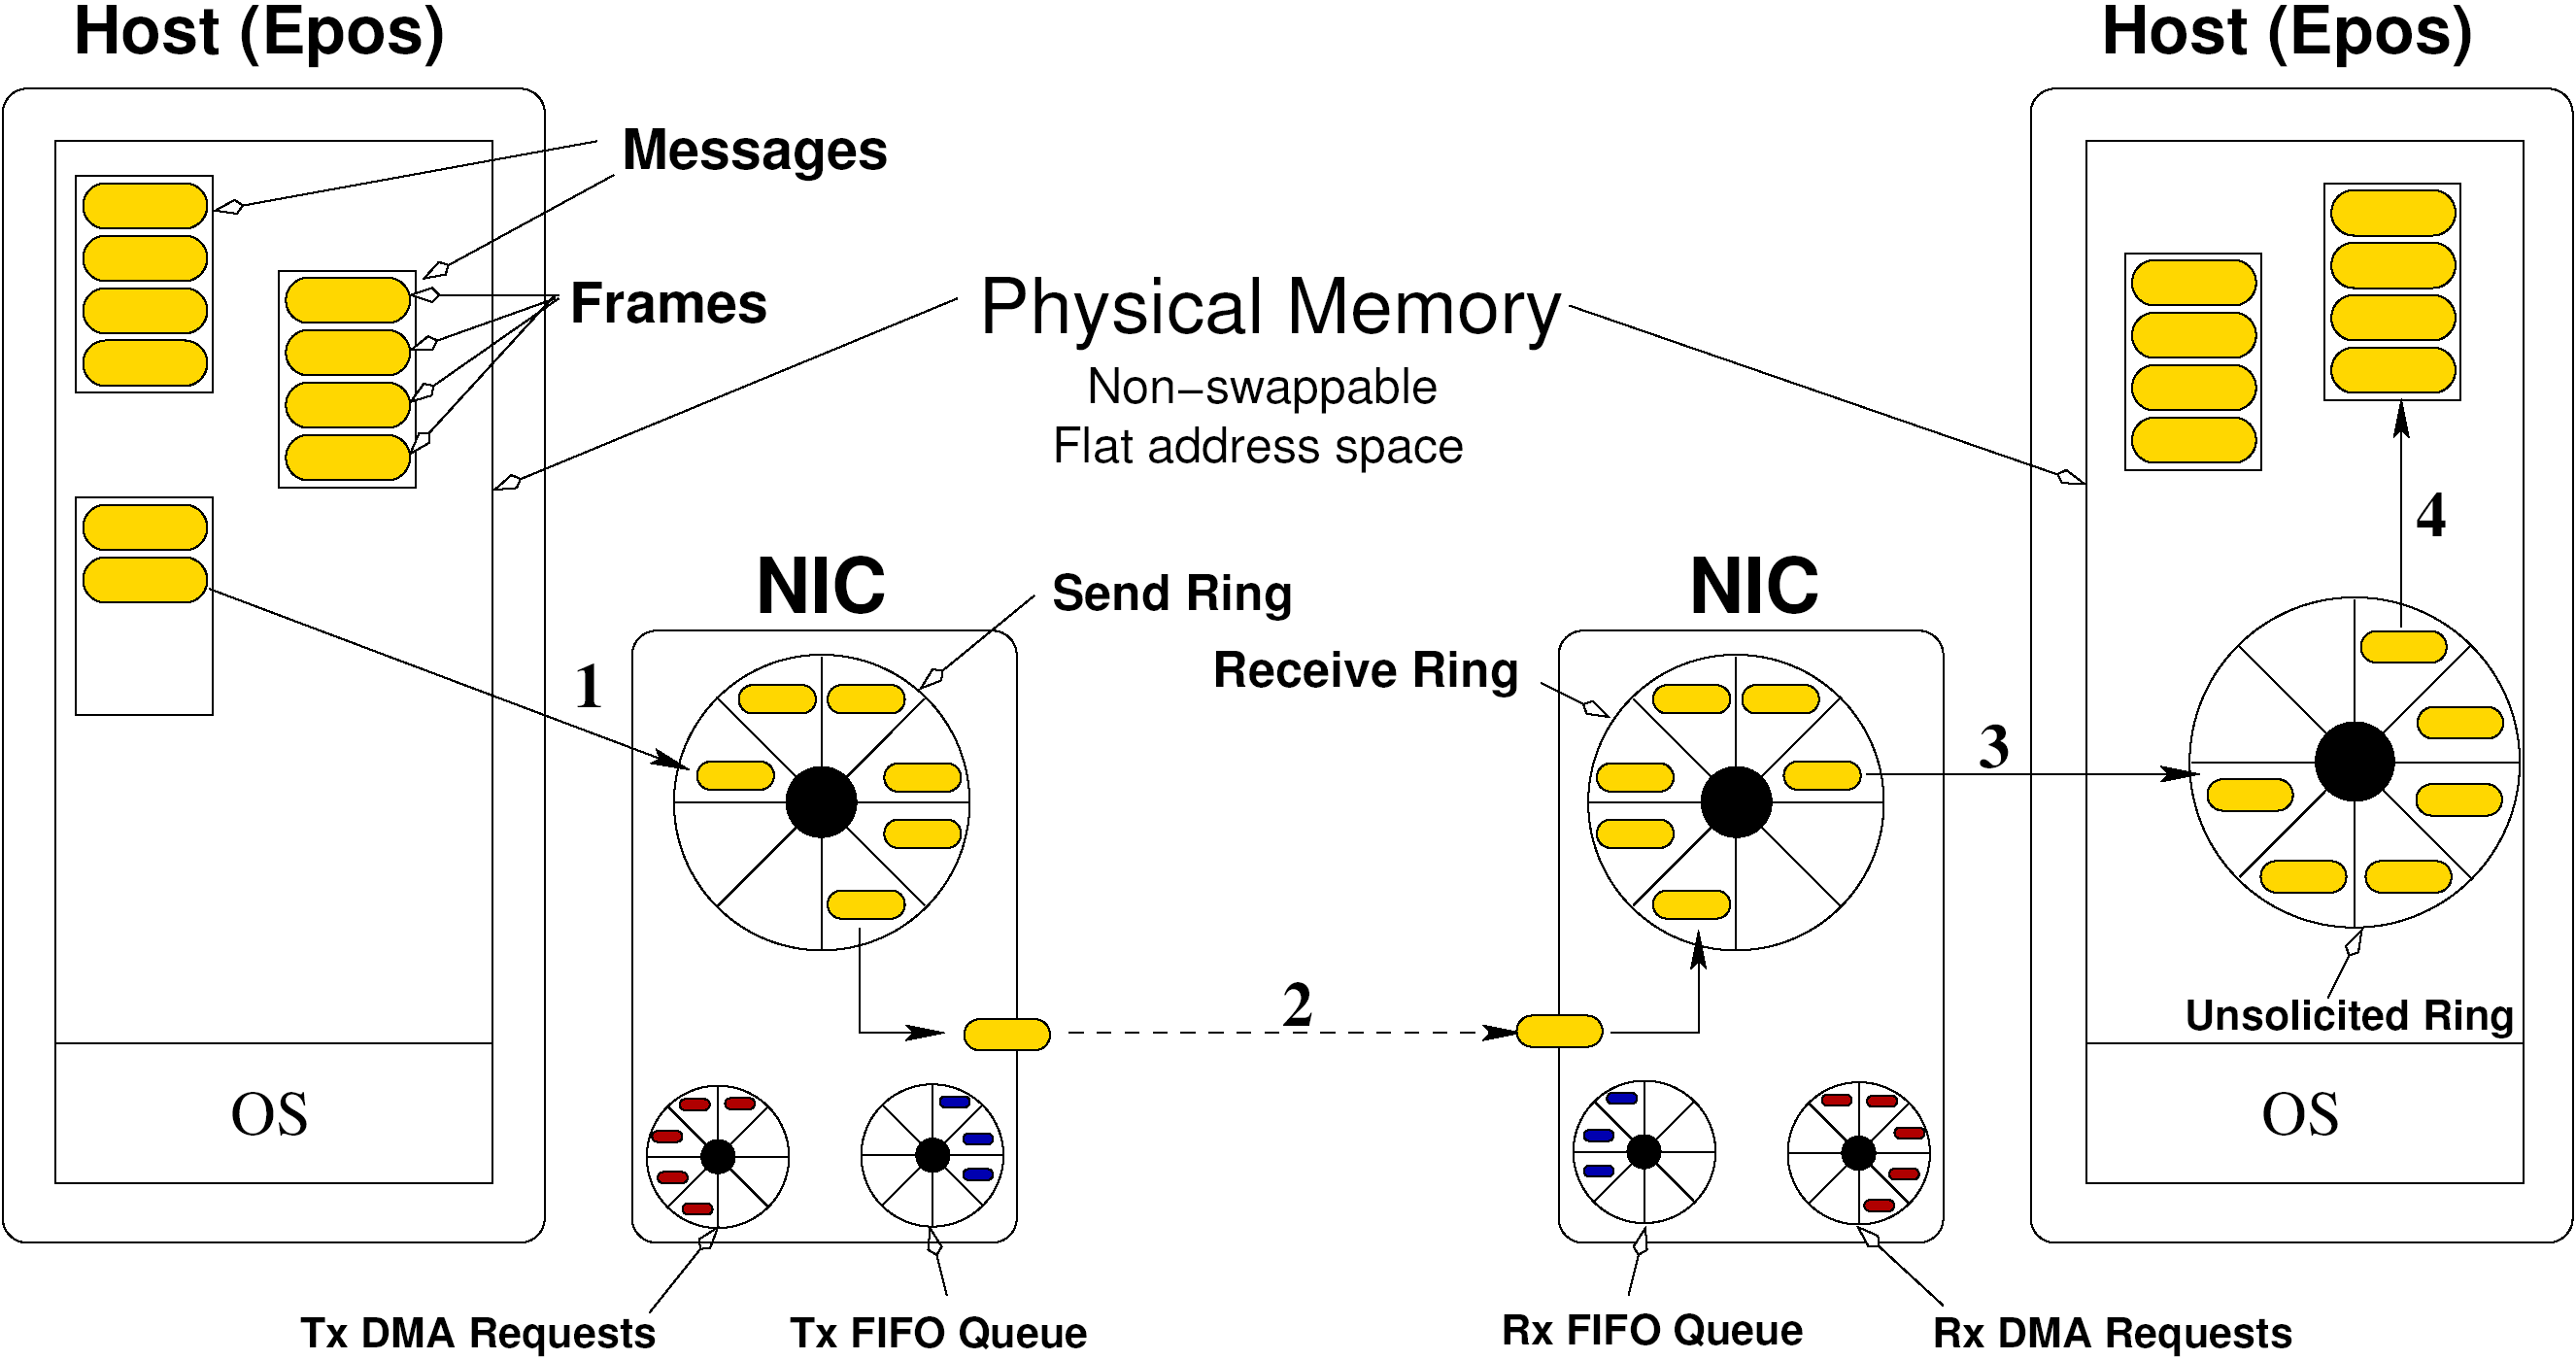
\includegraphics[scale=0.65]{fig/best_ever_design}}
\caption{The Myrinet Family baseline architecture.}
\label{fig:best_design}
\end{figure}

The NIC memory holds the six buffers that are used during communication. Send Ring and Receive Ring are circular buffers that hold the frames before they are accessed by the Network-DMA engine, the responsible for sending/receiving frames to/from the Myrinet network. Rx DMA Requests and Tx DMA Requests are circular chains of DMA control blocks, used by the Host-DMA engine for transferring frames between host and NIC memory. Rx FIFO Queue and Tx FIFO Queue are circular FIFO queues used by the host processor and LANai, Myrinet's network interface processor, to signal for each other the arrival of a new frame. The size of these buffers affects the communication performance and reliability and the choice of their sizes is influenced by the host's run-time system, memory space considerations, and hardware restrictions.

Much of the overhead observed in traditional protocol implementations is due to memory copies during communication. Some network technologies provide host-to-network and network-to-host data transfers, but Myrinet requires that all network traffic go through NIC memory. Therefore, at least three copies are required for each message: from host memory to NIC memory in the sending side, from NIC to NIC and from NIC memory to host memory in the receiving side. Write-combining, the DMA transfers start-up overhead and the fact that a DMA control block has to be written in NIC memory for each Host-DMA transaction make write PIO more efficient than DMA for small frames. The baseline architecture copies data from host to NIC using programmed I/O for small frames (less than 512 bytes) and Host-NIC DMA for large frames. Since reads over the I/O bus are much slower than writes, the baseline architecture uses DMA for all NIC-to-host transfers.

During communication, messages are split into frames of fixed size that are pushed into the communication pipeline. The frame size that minimizes the transmission time of the entire message in the pipelined data transfer is calculated \cite{frohlich-eposmyrinet} and the baseline architecture uses this value to fragment messages. Besides, the maximum frame size (MTU) is dynamically configurable. For each frame, the sender host processor uses write PIO to fill up an entry in the Rx DMA Requests (for large frames) or to copy (1) the frame directly to the Send Ring in NIC memory (for small frames). It then triggers a doorbell, creating a new entry in the Tx FIFO Queue and signaling for the LANai processor that a new frame must be sent. For large frames, the transmission of frames between host and NIC memory is carried out asynchronously by the Host/NIC DMA engine (1) and the frame is sent as soon as possible by LANai after the corresponding DMA finishes (2). Small frames are sent as soon as the doorbell is rung, since at this point the frame is already in NIC memory. A similar operation occurs in the receiving side: when a frame arrives from the network, LANai receives it and fills up an entry in the Rx DMA Requests DMA chain. The message is assembled asynchronously in the Unsolicited Ring circular buffer in host memory (3). The receiving side is responsible for copying the whole message from the Unsolicited Ring before it is overwritten by other messages (4). Note that specific protocol implementations can avoid this last copy using rendezvous-style communication, where the receiver posts a receive request and provides a buffer before the message is sent, a credit scheme, where the sender is requested to have credits for the receiver before it sends a packet, or even some other technique, achieving the optimal three copies.

The host memory layout is defined by the operating system being used. Besides, the Myrinet NIC impose some constraints on the usage of its resources that must be addressed by the OS. The most critical one relates to the Host/NIC DMAs: the Host-DMA engine can only access contiguous pages pinned in physical memory. Most communication systems implementations for Myrinet address this issue by letting applications pin/unpin the pages that contain its buffers on-the-fly during communication or by using a pinned copy block. The problem with these approaches is that they add extra overhead since pinning/unpinning memory pages requires system calls, which implies in context saving and switching, and using a pinned copy block adds extra data copies in host memory. In \textsc{Epos}, where swapping can be left out of the run-time system by mapping logical address spaces contiguously in physical memory, this issue does not affect the overall communication.

\begin{figure} [h]
\centering
\fbox{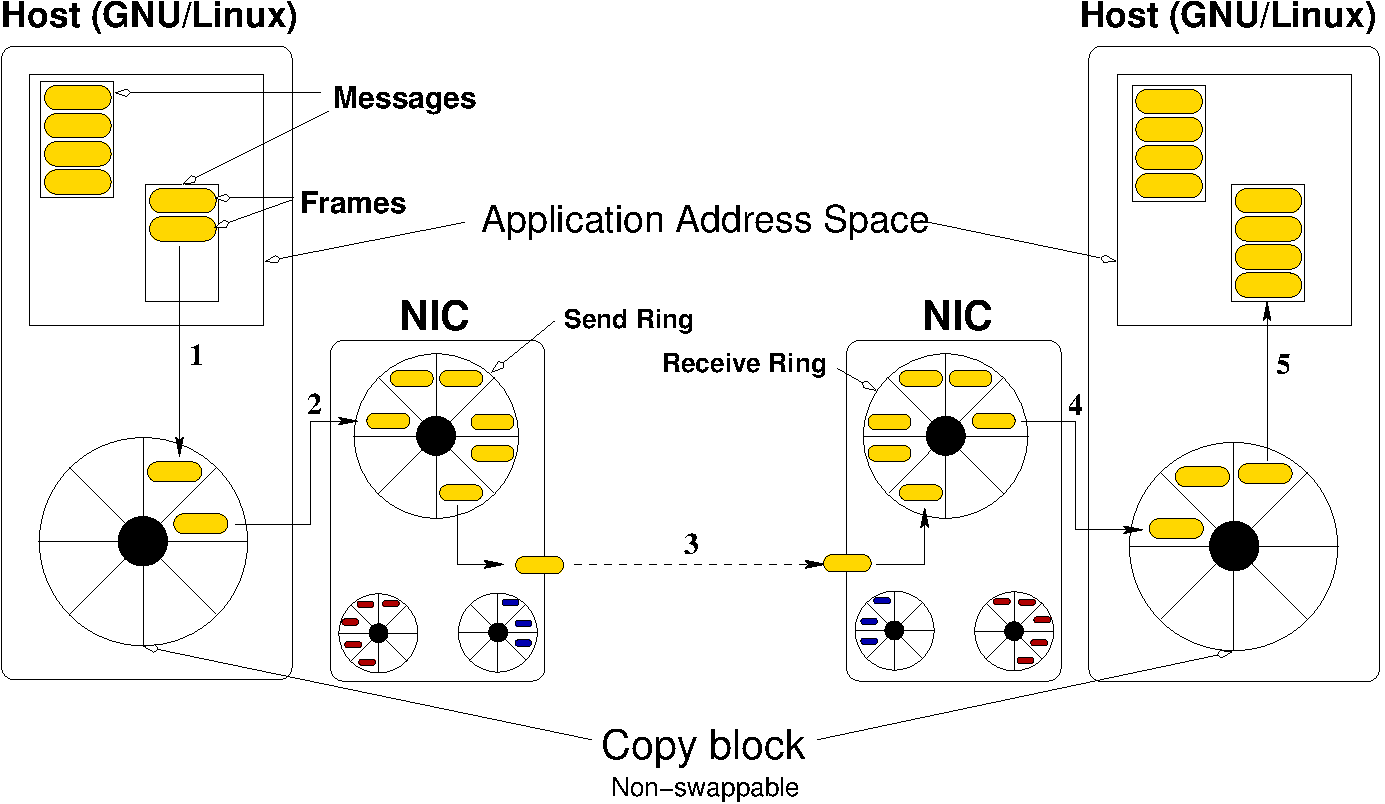
\includegraphics[scale=0.65]{fig/ever_design}}
\caption{The Myrinet Family baseline architecture in a GNU/Linux host.}
\label{fig:linux_design}
\end{figure}

Figure \ref{fig:linux_design} shows the memory layout and dynamic data flow of an implementation of the baseline architecture in a Myrinet GNU/Linux cluster. Issues such as address translation, kernel memory allocation and memory pinning had to be addressed in this implementation. Besides, a pinned copy block in kernel memory is used to interface Host/NIC DMA transfers, which adds one extra copy for each message in the sending side. Figure \ref{fig:linux_performance} exhibits a performance comparison between the GNU/Linux baseline architecture and the low-level driver GM (version 1.6.5), provided by the manufacturer of Myrinet. A round trip time test was performed in order to compare the two system's latency.

\begin{figure}[h]
\input graphs/GMxBaseline_graph.tex
\caption{Comparison between the baseline architecture's and GM's latency (in microseconds) for different frame sizes (in bytes).}
\label{fig:linux_performance}
\end{figure}

Many Myrinet protocols assume that the Myrinet network is reliable and, for that reason, no re-transmission or time-out mechanism is needed. Indeed, the risk of a packet being lost or corrupted in a Myrinet network is so small that reliability mechanisms can be safely left out of the baseline architecture. Alternative implementations that assume unreliable network hardware and recover from lost, corrupted, and dropped frames by means of time-outs, retransmission, and hardware supported CRC checks are addressed by specific protocol implementations since different application domains may need different trade off between reliability and performance.

The presented architecture may drop frames because of insufficient buffer space. The baseline architecture rests on a NIC hardware mechanism to partially solve this problem. Backpressure, Myrinet's hardware link-level flow control mechanism, is used to prevent overflow of network interface buffers, stalling the sender until the receiver is able to drain frames from the network. More sophisticated flow-control mechanisms must be provided by specific protocol implementations since specialized applications may only require limited flow-control from the network, performing some kind of control on their own.

%%%%%%%%%%%%%%%%%%%%%%%%%%%%%%%%%%%%%%%%%%%%%%%%%%%%%%%%%%%%%%%%%%%%%%%%%%%%%%%
\subsection{Myrinet low-level lightweight protocols}

While the baseline architecture is closely related to the underlying networking technology, low-level lightweight protocols are designed according to the communication requirements of specific classes of parallel applications. The lightweight protocols in the Myrinet family are divided into two categories: \emph{Infrastructure} and \emph{High-Performance} protocols.

\begin{description}

\item [Infrastructure protocols] provide communication services that were left out of the baseline architecture: transparent multicasting, QoS, connection management, protection schemes, reliable delivery and flow control mechanisms, among others. In order to keep latencies low it would be desirable to efficiently execute the entire protocol stack, up to the transport layer, in hardware. Programmable network interfaces can be used to achieve that goal. LANai makes the design of communication protocols more flexible. Infrastructure protocols exploit the network processor to the maximum, using more elaborate Myrinet control programs in order to offload a broader range of communication tasks to the LANai. The communication performance is affected due to the trade-off between performance and MCP complexity but for some specific classes of applications this is a small price to pay for the communication services provided.

\item [High-performance protocols] deliver minimum latency and maximum bandwidth to the run-time system. They usually consist in minimal modifications in the baseline architecture that are required by applications or in protocols that monitor the traffic patterns and dynamically modify the baseline architecture's customization points in order to address dynamic changes in application requirements.

\end{description}	

%%%%%%%%%%%%%%%%%%%%%%%%%%%%%%%%%%%%%%%%%%%%%%%%%%%%%%%%%%%%%%%%%%%%%%%%%%%%%%%
\section{Related Works\label{sec:related}}

There are several communication systems implementations for Myrinet, such as AM, BIP, PM, and VMMC, to name a few. Although these communication systems share some common goals, performance being one of them, they have made very different decisions in both the communication model and implementation, consequently offering different levels of functionality and performance. From the several published comparison between these implementations one can conclude that there is no single best low-level communication protocol since the communication patterns of the whole run-time system (application and run-time support) influences the impact of the low-level implementation decisions of a given communication system on applications' performance. Besides, run-time system specifics greatly influences communication system implementations' functionality.

While the Myrinet communication systems mentioned above try to deliver a generic, all-purpose solution for low-level communication, the main goal of the presented research is customization of low-level communication software. The architecture we propose should be flexible enough to allow that a broad range of the implementation decisions behind each one of the several Myrinet communication systems be supported as a lightweight protocol.

Although our work has focused on Myrinet, there are some other networks for which the same concepts can be applied. Cluster interconnection technologies that are also implemented with a programmable NIC that can execute a variety of protocol tasks include DEC's Memory Channel, the interconnection network in the IBM SP series and Quadrics' QsNet.

%%%%%%%%%%%%%%%%%%%%%%%%%%%%%%%%%%%%%%%%%%%%%%%%%%%%%%%%%%%%%%%%%%%%%%%%%%%%%%%
\section{Conclusions\label{sec:end}}

The widespread of cluster systems brings up the necessity of improvements in the software environment used in cluster computing. Cluster system software must be redesigned to better exploit clusters' hardware resources and to keep up with applications' requirements. Parallel-programming environments need to be developed with both the cluster and applications efficiency in mind. 

In this paper we outlined the design of an application-oriented communication sub-system based in low-level lightweight protocols for the Myrinet networking technology. The design decision related to these protocols' baseline communication architecture were discussed and a GNU/Linux implementation was presented. Experiments are being carried out to determine the best values for the architecture's customization points in different traffic pattern conditions.

In order to design an efficient, application-oriented communication system for clusters it is necessary to better understand the relation between the design decisions in low-level communication software and the performance of high-level applications. We intend to evaluate how different low-level communication schemes impact applications performance, using different low-level communication protocols and real parallel applications, since commonly used benchmarks fail in represent applications' communication patterns. The redesign of \textsc{Epos} communication system was a first step towards that goal.

%%%%%%%%%%%%%%%%%%%%%%%%%%%%%%%%%%%%%%%%%%%%%%%%%%%%%%%%%%%%%%%%%%%%%%%%%%%%%%%
\bibliographystyle{plain}
\bibliography{os,cluster,parallel,network,guto,draftbib}

\end{document}


The proposed baseline architecture provides no protection. However, protection mechanism can be easily implemented over the baseline architecture since Myrinet's doorbell region can be divided between several user-processes. However, multiplexed usage of the described architecture would require that each user-process had its own dma chains in NIC memory. Because network interface memory is small, only a limited number of user process can play

, which works just fine in a dedicated high-performance environment, where there is always only one application being executed at a time. Unless explicitly implemented by a network interface lightweight protocol, the NIC hardware can not be multiplexed.

control transfer - polling to detect incoming messages Polling the network interface card for incoming messages; Avoid system calls for communication; write a flag in chached host memory (using DMA) when a frame is available. The host polls by reading its local memory (usually cached since polls happen very frequently)
the lanai DMAs the dma block to host memory shared flag polled by the main processor or via interruptions.

The architecture supports only point-to-point messages.
Finally, comunicacao ponto a ponto nao protegida por sessoes in order (FIFO) message delivery
multicast is desirable since its a fundamental component of collective communication operations. and can be implemented on top of point-to-point messages. 



Being fruit of \emph{Application-Oriented System Desing}~\cite{Froehlich:2001}, \textsc{Epos} features a highly customizable communication system. This communication system was already partially implemented for some network technologies, including \emph{Ethernet} and \emph{Myrinet}~\cite{Froehlich:ccgrid:2001}. However, little attention was given to the originally proposed family of \emph{lightweight communication protocols} until now. **We present the latest advances in developing those protocols** as well as a novel baseline architecture for the new generation of \emph{Myrinet} network adapters. 

%%%%%%%%%%%%%%%%%%%%%%%%%%%%%%%%%%%%%%%%%%%%%%%%%%%%%%%%%%%%%%%%%%%%%%%%%%%%%%%
\section{Overview of the Myrinet technology\protect\footnote {Myrinet-2000-Fiber/PCI64B series.}}

A deep understanding of the network technology in question, from the network interface card (NIC) architecture to the routing mechanisms involved, becomes necessary. This section gives an overview of the Myrinet networking technology and describes in depth the network features used in the baseline architecture of the Myrinet family.

Myricom's Myrinet is a switched, gigabit-per-second system area network (SAN). The ANSI standard Myrinet-on-VME Protocol Specification \cite{myrinetvita} defines packets of variable length that are wormhole-routed through a network of highly reliable links and crossbar switches. Figure 
\ref{fig:host_nic_interface} shows the architecture of a node in a Myrinet (SAN).

\begin{figure} [h]
\centering
\fbox{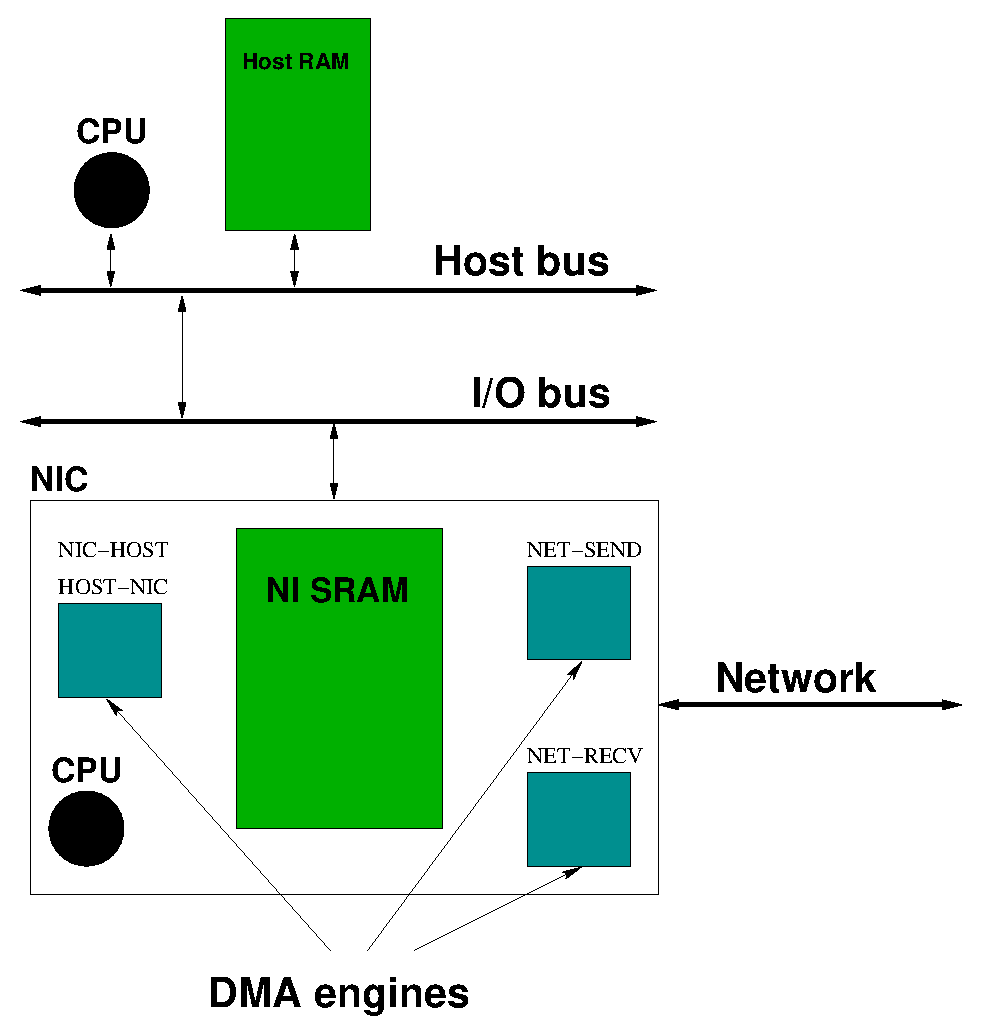
\includegraphics[scale=0.6]{fig/host_nic_interface}}
\caption{Architecture of a node in a Myrinet SAN.}
\label{fig:host_nic_interface}
\end{figure}

Each node has a Myrinet NIC connected to its I/O bus, a typical organization for commodity hardware. The Myrinet NIC is a programmable communication device that provides an interface to the Myrinet SAN. It is equipped with an instruction-interpreting on-board RISC processor, called LANai, a set of DMA engines and on-board fast SRAM.

Myrinet requires that all incoming and outgoing packets go through NIC memory during communication, which makes of the relatively small amount of SRAM a precious resource. The on-board memory holds all code and data for the LANai processor, the temporary buffers for the incoming and outgoing packets and other data used during communication. A host can access its network interface's memory using programmed I/O (PIO) and both the host and the NIC can use DMA to access data in each other's memory. The NIC allows at most two memory accesses per clock cycle, assigned based on the following priority order (highest to lowest): host (programmed I/O), net-recv DMA, net-send DMA, and the LANai processor.

LANai gives protocols designers a great flexibility since part of the communication can be offloaded from the host CPU to the NIC processor. Besides, the NIC processor can be programmed to provide a variety of special communications services closer to the hardware. LANai is much slower than the host CPU, which yields a trade-off between performance and complexity of the communication tasks executed by it. Besides, Myrinet control programs (MCP) must be carefully designed since adding just a few instructions to the critical path of the MCP affects communication performance.

Three DMA engines are provided by the Myrinet NIC. They are responsible for injecting a frame into the network (Net-Send), for consuming a frame off of the network (Net-Recv) and for data transfers between host and NIC (Host/NIC). These DMA engines are designed to work fully in parallel in order to improve communication performance. The number of DMA operations that can be executed concurrently is limited by the restriction in the number of memory access per cycle imposed by the NIC.

In addition to that, Myrinet networks provide other features that can be exploited in many different ways by the communication protocols:

\begin{description}

\item [DMA queuing:] Host/NIC data transfer requests can be queued together and executed asynchronously by the Host/NIC DMA engine. The engine uses up to four chains of DMA control blocks stored in LANai memory to trigger DMA-mastering operations. Each one of these chains can be activated by the host or the LANai. When a chain is activated, the Host/NIC DMA engine executes a host/NIC data transfer for each block in that chain until it finds a terminal block, when it waits until that chain is reactivated. Multiple reactivations of a chain already active is harmless. The DMA engine processes chains in priority order. For example, if the DMA engine is executing the DMA operation described in a control block in the lowest priority chain when a new control block is queued in a higher priority chain, the DMA engine will finish the DMA operation being executed and move to that higher priority chain. A control block can be configured to make the Host/NIC DMA engine signal when it completes the DMA operation for that block.

\item [Hardware doorbell mechanism:] The Myrinet NIC implements a mechanism that allows the host to write anywhere in a specified region of the NIC I/O address space, the doorbell region, and to have that data stored into a FIFO queue in the LANai memory. The I/O address accessed by the host is also written in the FIFO queue.

\item [Backpressure flow control:] Hop-by-hop flow control scheme employed by Myrinet that stalls the sending NIC if the receiver is not available. One drawback of backpressure is the possibility of creating deadlock situations. There is a time limit in the backpressure mechanism that can be dynamically configured by software and is used to prevent deadlocks: if the receiver does not drain the network within the specified time limit the network resets the NIC or truncates the packet.

\item [Wormhole Routing:] In wormhole routing networks, each intermediate switch forwards a packet to the desired output port as soon as it enters the switch, without waiting for the entire packet to be assembled.

\end{description}

